\usepackage[T1]{fontenc}
\usepackage[utf8]{inputenc}
\usepackage[ngerman]{babel}
\usepackage{tikz} % venn diagram
% \usepackage{enotez} % image sources (instead of endnotes for linking)
\usepackage{pgfplotstable} % csv to table
\usepackage[style=apa,backend=biber,natbib]{biblatex}
\usepackage{bookmark}
\usepackage{svg} % includesvg

% currentname
\usepackage{nameref}
\makeatletter
\newcommand*{\currentsectionname}{\@currentlabelname}
\makeatother

% load TUC templates, set color scheme to IF
\usetheme[fakcolor=if]{tuc2019}
\mode<article>{\usepackage{beamerarticletuc2019}}

\addbibresource{bibliography.bib}
\usetikzlibrary{calc}
\usepgfplotslibrary{statistics} % Boxplots

% colors
\definecolor{s4d-blue}{HTML}{055DA9}
\definecolor{plot1}{HTML}{8DC144}
\colorlet{plot2}{s4d-blue}
\definecolor{plot3}{HTML}{84689B}
\definecolor{plot4}{HTML}{CF461C}

% deactivate navigation
\setbeamertemplate{navigation symbols}{}

% metadata
\newcommand{\Title}{Bachelorarbeit: Blockbasierte Daten-Konvertierung}
\newcommand{\ShortTitle}{Blockbasierte Daten-Konvertierung}
\newcommand{\ShortSubTitle}{Einschätzung der empfundenen Produktivitätssteigerung }
\title[\ShortTitle]{\Title}
\subtitle{\ShortSubTitle{} im Umgang mit Umweltdaten}
\author{Joshua Jeschek}
\date{16. Oktober 2024}
\institute[TUC]{TU Chemnitz}
\titlegraphic{
\includegraphics[height=0.19\textheight]{tuc2019/logo/tuc_green}}
% \tucurl{}

\newcommand{\Note}[1]{\note{\begin{itemize}#1\end{itemize}}}

\begin{document}
\tucthreeheadlines{}
\begin{frame}
  \titlepage{}

  \Note{
      \item wie Titel verrät entstammt die Motivation aus dem Bereich der Umweltdaten, also möchte ich auch damit anfangen diese Motivation kurz darzustellen
  }

\end{frame}

\begin{frame}

  \begin{itemize}
    \item Große Komplexität im Bereich der Umweltdaten.\\($m \times n$ Transformationen)
    \item Starke Vereinfachung durch Sekundärsystem Simplex4TwIS.\\($m + n$ Transformationen)
  \end{itemize}

  \newtheorem{pro}{Problemstellung}
  \begin{pro}
    \begin{itemize}
      \item Weiterhin wird manuelle Eingabe von SQL benötigt.
      \item Kompliziert für Fachexpert:innen ohne technische Kenntnisse.
      \item Anfällig für Tippfehler.
      \item Struktur der Eingangsdaten muss bekannt sein.
    \end{itemize}
  \end{pro}

  \Note{
    \item Komplexität durch viele Primärsysteme, die Daten erfassen und heterogene Datensätze erzeugen
    \item viele Formate, sowohl in Eingangsdaten als auch Ausgabeformate
    \item Ausgabeformate müssen oft Daten aus verschiedenen Bereichen kombinieren, komplexe Datentransformationen ($m \times n$, jedes Eingangsformat könnte in jedem Ausgabeformat benötigt werden)
    \item Sekundärssystem Simplex4TwIS vereinfacht,
    \item harmonisierte Speicherung, ermöglicht wiederholbare Imports und Exports, $m$ Importe, $n$ Exporte \textrightarrow $m + n$
  }

\end{frame}

\begin{frame}

  \newtheorem{goal}{Zielsetzung}
  \begin{goal}
    \begin{itemize}
      \item Entwicklung eines Block-Editors.
      \item Durchführung einer Usability-Studie.
    \end{itemize}
  \end{goal}

\end{frame}

\tuctwoheadlines{}
\subsection*{\ShortTitle}
\begin{frame}
  \frametitle{Gliederung}
  \tableofcontents

  \note{
    \begin{itemize}
    \end{itemize}
  }

\end{frame}

\section{Theoretische Grundlagen}
\subsection{Simplex4TwIS}

\begin{frame}
  \frametitle{\currentsectionname}

  \begin{figure}
    \tikzstyle{s4dArrow}=[->, line width=1.5mm, s4d-blue]
\centering
\resizebox{.95\textwidth}{!}{%
  \begin{tikzpicture}
    \node (s4dImg) at (8, -6)
    [inner sep=0, outer sep=0]
    {
\includegraphics[height=4cm]{assets/s4t.png}};

    \node (s4d) at ($(s4dImg.center) + (0.15,0)$)
    [align=center, minimum width=3.1cm, minimum height=4.25cm]
    {};

    \node (s4dReality) at (s4d.north east)
    [anchor=south east, align=center]
    {\huge Realitäts-\\\huge modell};

    \node (s4dImport) at ($(s4d.west) - (5,0)$)
    [anchor=east, align=center]
    {\huge Import};

    \node (s4dScenarios) at ($(s4d.east) + (5,0)$)
    [anchor=west, align=center, minimum width=3.5cm]
    {\huge Simplex\\\huge Szenarios};

    \node (s4dService) at (s4dScenarios |- s4dReality.base)
    [anchor=base, align=center, minimum width=3.5cm]
    {\huge Simplex\\\huge Service};

    \draw [s4dArrow]
    (s4dImport) edge node (importArrow) {} (s4d)
    (s4d) edge node (scenarioArrow) {} (s4dScenarios)
    (s4dReality) edge (s4dService)  (s4dScenarios) edge (s4dService);

    \node (block1) at ($(importArrow.center) - (0,2)$)
    [align=center]
    {\Large Konvertierung zu\\\Large Realitätsmodell};

    \node (block2) at ($(scenarioArrow.center) - (0,2)$)
    [align=center]
    {\Large Zusammenstellung von\\\Large Anwendungsfällen};

    \node (importCircle) at (s4dImport.center)
    [shape=circle, minimum width=7cm]
    {};

    \node (i1) at (importCircle.140) {\Large{}.shp};
    \node (i2) at (importCircle.160) {\Large{}.json};
    \node (i3) at (importCircle.180) {\Large{}.csv};
    \node (i4) at (importCircle.200) {\Large{}API};
    \node (i5) at (importCircle.220) {\Large{}\dots};

    \draw [s4dArrow, line width=.5mm]
    (i1) edge (s4dImport)
    (i2) edge (s4dImport)
    (i3) edge (s4dImport)
    (i4) edge (s4dImport)
    (i5) edge (s4dImport);

  \end{tikzpicture}
}

    \caption{Datenverarbeitung in Simplex4TwIS.}
  \end{figure}

  \Note{
    \item betrachten Simplex4TwIS aus Sicht der Daten, sieht so aus
    \item Aus verschiedenen Dateiformaten
  }

\end{frame}

\begin{frame}
  \frametitle{Realitätsmodell}

  \begin{itemize}
    \item Objektorientiertes und graphenbasiertes Datenmodell.
    \item \textbf{Harmonisiert}: Objekte, Attribute und Verbindungen besitzen immer gleiche Datenstrukturen.
    \item \textbf{Atomar}: Jede Dateneinheit wird als Objektklasse abgebildet.
  \end{itemize}

  \Note{
    \item Standardfelder: Schlüssel immer gleich, können jedoch durch zusätzliche Metadaten wie Name und Kommentar weiter beschrieben werden
    \item zusätzliche Informationen über Sachattribute, welche in den Metadaten über Standardfelder beschrieben werden
    \item Datenmodell orientiert sich nicht an fachspezifischen Anforderungen
    \item anwendungsspezifische Auswertungen basierend auf Realitätsmodell führen dazu dass keine fachspezifischen Modelle mehr benötigt werden
    \item Bereitstellung der Daten über API-Features Dienst (zurück klicken)
  }

\end{frame}

\begin{frame}
  \frametitle{Laden \& Konvertieren}

  \begin{itemize}
    \item Verschiedene Dateiformate und API-Features-Dienste können in Datenbanktabellen geladen werden.
    \item Konvertierungen werden genutzt, um aus den Tabellen einzelne Objekte im Realitätsmodell zu erstellen.
    \item Dazu werden für jedes Eingangsformat \textit{Konvertierungsvorschriften} benötigt.
  \end{itemize}

  \Note{
    \item Laden von verschiedenen Dateiformaten (CSV, JSON, SHP) oder API-Diensten (API-Features) in Datenbanktabellen
    \item Dabei werden Daten in einzelne Bestandteile zerlegt
    \item Dann Erstellen von Konvertierungen, die aus den Tabellen einzelne Objekte gemäß des Realitätsmodell auslesen
    \item Dazu muss eine Konvertierungsvorschrift definiert werden
    \item Das sind die $m$ Importe vom Anfang
    \item Das soll durch den entwickelten Block-Editor vereinfacht werden
    \item nach dem Laden existieren Objekte in Realitätsmodell, API Dienst
    \item sind also schon nach diesem Schritt zugänglich, ohne sie weiter für Export vorbereiten zu müssen
    \item \textrightarrow ABER wenn komplexe Auswertung benötigt werden, SimplexSzenarios
  }

\end{frame}

\begin{frame}
  \frametitle{SimplexSzenarios}

  \begin{itemize}
    \item Zusammenstellung von Daten im Realitätsmodell zu fachspezifischen Auswertungen und standardisierten Formaten.
    \item Für jedes Ausgabeformat werden \textit{Bildungsvorschriften} benötigt.
  \end{itemize}

  \Note{
    \item Dazu können mehrere Klassen aus dem Realitätsmodell gleichzeitig abgefragt werden, basierend auf den bestehenden Verbindungen
    \item Umsetzung von Berechnungen
    \item Bedienen von standardisierten Formaten
    \item Bereitstellung über API-Features Dienst
  }

\end{frame}

\begin{frame}
  \frametitle{SimplexService}

  \begin{itemize}
    \item \textbf{API - Features}: API-Standard für Geodaten vom Open Geospatial Consortium.
    \item Wird von Simplex4TwIS genutzt, um Daten des Realitätsmodells und SimplexSzenarios auszugeben.
    \item Für den Block-Editor werden Teile des Entwurfs "OGC API - Features - Part 3: Filtering" genutzt:
          \begin{itemize}
            \item Common Query Language (CQL)
            \item Funktionen
            \item Queryables
          \end{itemize}
    % \item Objekt- und Verbindungsklassen im Realitätsmodell werden in der API als \textit{collections} ausgegeben, Objekte und Verbindungen sind deren \textit{items}.
  \end{itemize}

\end{frame}

\subsection{OGC API - Features}
\begin{frame}
  \frametitle{\currentsectionname}

  \note{
    \begin{itemize}
    \end{itemize}
  }

\end{frame}

\subsection{Verwandte Arbeiten}
\begin{frame}
  \frametitle{\currentsectionname}

  % \note{
  %   \begin{itemize}
  %   \end{itemize}
  % }

\end{frame}

\begin{frame}
  \frametitle{DataSnap}

  \begin{minipage}{.6\textwidth}
    \begin{itemize}
      \item Weiterentwicklung von \textit{Snap!}, die an Fachexpert:innen gerichtet ist.
      \item Einfaches Importieren von Daten.
      \item Nutzung von externen Rechnern zur Beschleunigung der Auswertung.
      \item Benutzung von \textit{Snap!}-Blöcken zur Definition der Datenverarbeitung.
    \end{itemize}
  \end{minipage}%
  \begin{minipage}{.4\textwidth}
    \begin{figure}
      \begin{center}
        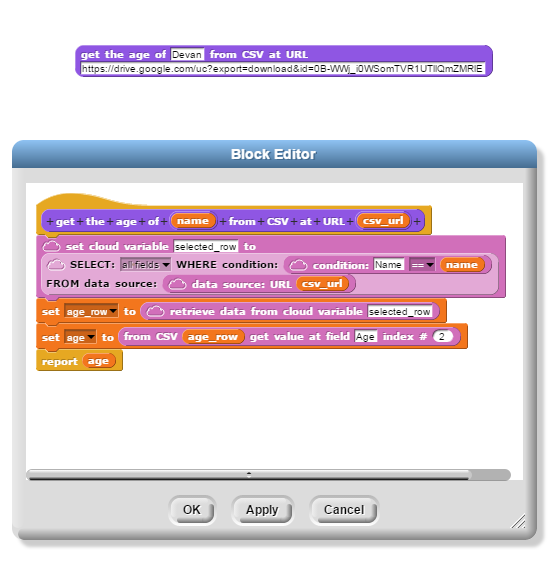
\includegraphics[width=0.95\textwidth]{assets/datasnap-block-definition.png}
      \end{center}
      \caption{Definition eines Blocks in \textit{DataSnap}. \parencite[26]{hellmannDataSnapEnabling2015}}
    \end{figure}
  \end{minipage}

  \Note{
    \item Masterarbeit
    \item Importieren über diesen dunkelpinken Block "data source"
    \item Abspeichern in sog. cloud variablen - auf externem Rechner, also Server
    \item auf dem Server können dann auch Berechnungen ausgeführt werden, weniger abhängig vom Client
    \item Hier rechts wird die Funktionalität als Block definiert, um später in anderen Abfragen schnell wiederverwendet zu werden
  }

\end{frame}

\begin{frame}
  \frametitle{DataSnap (cont.)}

  \begin{itemize}
    \item Visualisierung der Ergebnisse.
  \end{itemize}
  \begin{figure}
    \begin{center}
      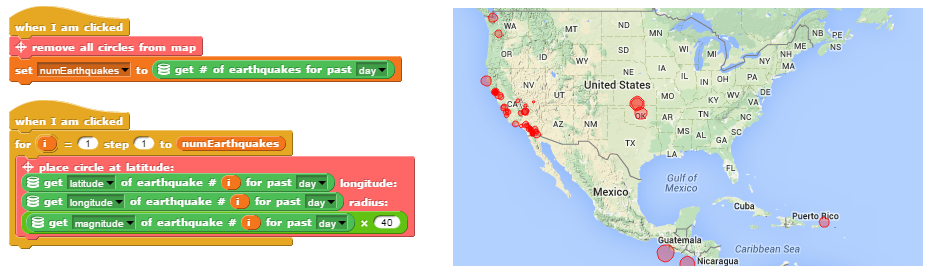
\includegraphics[width=0.95\textwidth]{assets/datasnap-visualization.png}
    \end{center}
    \caption{Visualisierung von Erdbeben mit \textit{DataSnap}. \parencite[28]{hellmannDataSnapEnabling2015}}
  \end{figure}

  \Note{
    \item mithilfe von standard Snap! und neu eingeführten Blöcken Visualisierung möglich
    \item Hier z.B. Erdbeben in Nordamerika mit Darstellung der Magnitude in Form des Radius der Kreise
  }

\end{frame}

\section{Entwicklung und Usability-Studie}
\subsection{Block-Editor}
\begin{frame}
  \frametitle{\currentsectionname}

  \note{
    \begin{itemize}
    \end{itemize}
  }

\end{frame}

\subsection{Usability-Studie}
\begin{frame}
  \frametitle{\currentsectionname}

  \note{
    \begin{itemize}
    \end{itemize}
  }

\end{frame}

\subsection{Erkenntnisse}

\begin{frame}
  \frametitle{\currentsectionname}

  \begin{itemize}
    \item Der Editor wurde als Vereinfachung der Abläufe empfunden.
    \item Tipp- und Syntax-Fehler konnten vermieden werden, semantische Fehler traten selten auf.
    \item Alle Teilnehmer:innen fühlten sich mit dem Block-Editor effizienter als zuvor, da z.B. häufiges Nachschlagen entfällt.
  \end{itemize}

  \Note{
    % \item CTA hat meistens gut funktioniert
    \item eine Person äußerte sich freudig darüber nun solche Aufgaben auch selbst durchführen zu können
    \item Grund für Effizienz auch Auswahlmenü, verhindert häufiges Nachschlagen
  }

\end{frame}

\begin{frame}
  % \frametitle{\currentsectionname{} (cont.)}

  \begin{figure}
    \pgfplotstableread[col sep=comma]{assets/study-results.csv}\datatable
\centering
\resizebox{.95\textheight}{!}{%
  \begin{tikzpicture}
    \begin{axis}[
        boxplot/draw direction=y,
        boxplot/every median/.style={ultra thick},
        xtick={1,2,3},
        xticklabels={Szenario 1, Szenario 2, Szenario 3},
        ytick={1,...,7},
        ymin=1,
        ylabel={SEQ},
      ]
      \addplot+ [boxplot, plot1] table [y=a] {\datatable};
      \addplot+ [boxplot, plot2] table [y=b] {\datatable};
      \addplot+ [boxplot, plot3] table [y=c] {\datatable};
    \end{axis}
  \end{tikzpicture}
}

    \caption{Antworten auf die Single Ease Question nach jedem Szenario (1: sehr schwer, 7: sehr einfach).}
  \end{figure}

  \Note{
    \item bevor wir auf Details eingehen erstmal nachschauen was so die quantitativen Daten sagen, die haben dann meistens zu Gesprächen geführt die ins Detail gehen
    \item erstes Szenario einfache Zuordnung, wurde als am einfachsten eingeschätzt
    \item Szenario 2 und 3 ungefähr ähnlich eingeschätzt, aber bei Szenario 3 gingen Meinungen weiter auseinander, könnte an unterschiedlichen Erfahrungsständen und Vertrautheit mit Konzept von SimplexSzenario liegen
  }

\end{frame}

\begin{frame}
  % \frametitle{\currentsectionname{} (cont.)}

  \begin{figure}
    \pgfplotstableread[col sep=comma]{assets/study-results.csv}\datatable
\centering
\resizebox{.95\textheight}{!}{%
  \begin{tikzpicture}
    \begin{axis}[
        boxplot/draw direction=y,
        boxplot/every median/.style={ultra thick},
        xtick={1,2},
        xticklabels={Vorversion, Block-Editor},
        ytick={1,...,10},
        ymin=1,
        ylabel={Einfachheit der Benutzung},
      ]
      \addplot+ [boxplot, plot1] table [y=prev] {\datatable};
      \addplot+ [boxplot, plot2] table [y=ges] {\datatable};
    \end{axis}
  \end{tikzpicture}
}

    \caption{Einschätzung der Einfachheit der Benutzung nach dem Usability Test auf einer Skala von 1 (sehr schwer) bis 10 (sehr einfach).}
  \end{figure}

  \Note{
    \item deutlich zu erkennen, dass Block-Editor besser als die Vorversion eingeschätzt wird
  }

\end{frame}

\begin{frame}
  % \frametitle{\currentsectionname{} (cont.)}

  \begin{figure}
    \colorlet{presentation}{plot1}
\colorlet{interaction}{plot2}
\colorlet{content}{plot3}
\colorlet{technical}{plot4}
\centering
\resizebox{.75\textheight}{!}{%
  \begin{tikzpicture}
    \begin{axis}[
        xbar=0pt,
        xmajorgrids=true,
        xtick={0,...,10},
        xmin=0,
        xmax=6,
        xlabel={Absolute Häufigkeit},
        /pgf/bar shift=0pt,
        legend style={legend cell align=left},
        legend pos=south east,
        axis y line*=none,
        axis x line*=bottom,
        tick label style={font=\footnotesize},
        legend style={font=\footnotesize},
        label style={font=\footnotesize},
        width=.6\textwidth,
        bar width=3.5mm,
        ymin=1,
        ytick={1,...,20},
        ytick style={draw=none},
        yticklabels={
            {Übersichtlichkeit Funktionsliste},
            {Präfix von Objektklassen},
            {Details zu Funktionen},
            {Benennung Abfragbare Felder},
            {Probleme mit Scrollen},
            {Zugriff auf die Quelldaten},
            {Automatische Typ-Filterung},
            {Angabe von statischen Werten},
            {Auswahl von Überladungen},
            {Benennung rechter Bereich},
            {Benennung des Speichern-Buttons},
            {Parameterübernahme bei Überladungen},
            {Drag and Drop},
            {Ersetzen von Einträgen},
            {Details zu Parametern},
            {Metadaten von Szenario-Feldern},
            {Anzeige von Attributen in Ziel},
            {Datentyp von Szenario-Feldern},
            {Symbole für Datentypen},
            {Bedienreihenfolge von Funktionen},
          },
        area legend,
        y=6mm,
        enlarge y limits={abs=0.625},
        every axis plot/.append style={fill}
      ]
      \addplot[interaction]  coordinates {(0,0)};  \addlegendentry{Interaktion (8)}
      \addplot[presentation] coordinates {(0,0)};  \addlegendentry{Darstellung (7)}
      \addplot[content]      coordinates {(0,0)};  \addlegendentry{Inhalt (4)}
      \addplot[technical]    coordinates {(0,0)};  \addlegendentry{Technisch (1)}

      \addplot[presentation] coordinates {(1,1)};  % Übersichtlichkeit Funktionsliste
      \addplot[content]      coordinates {(2,2)};  % Präfix von Objektklassen
      \addplot[content]      coordinates {(2,3)};  % Details zu Funktionen
      \addplot[presentation] coordinates {(2,4)};  % Benennung Abfragbare Felder
      \addplot[technical]    coordinates {(3,5)};  % Probleme mit Scrollen
      \addplot[content]      coordinates {(3,6)};  % Zugriff auf die Quelldaten
      \addplot[interaction]  coordinates {(3,7)};  % automatische Typ-Filterung
      \addplot[interaction]  coordinates {(3,8)};  % Angabe von statischen Werten
      \addplot[interaction]  coordinates {(3,9)};  % Auswahl von Überladungen
      \addplot[presentation] coordinates {(4,10)}; % Benennung rechter Bereich
      \addplot[presentation] coordinates {(4,11)}; % Benennung des Speichern-Buttons
      \addplot[interaction]  coordinates {(4,12)}; % Parameterübernahme bei Überladungen
      \addplot[interaction]  coordinates {(4,13)}; % Drag and Drop
      \addplot[interaction]  coordinates {(4,14)}; % Ersetzen von Einträgen
      \addplot[content]      coordinates {(5,15)}; % Details zu Parametern
      \addplot[presentation] coordinates {(5,16)}; % Metadaten von Szenario-Feldern
      \addplot[presentation] coordinates {(5,17)}; % Anzeige von Attributen in Ziel
      \addplot[interaction]  coordinates {(5,18)}; % Datentyp von Szenario-Feldern
      \addplot[presentation] coordinates {(6,19)}; % Symbole für Datentypen
      \addplot[interaction]  coordinates {(6,20)}; % Bedienreihenfolge von Funktionen
    \end{axis}
  \end{tikzpicture}
}

    \caption{Häufigkeit des Auftretens verschiedener Usability-Probleme.}
  \end{figure}

\end{frame}

\begin{frame}

  \begin{itemize}
    \item Verwirrungen bezüglich der Bedienreihenfolge der Funktionen.
  \end{itemize}

  \begin{figure}
    \begin{center}
      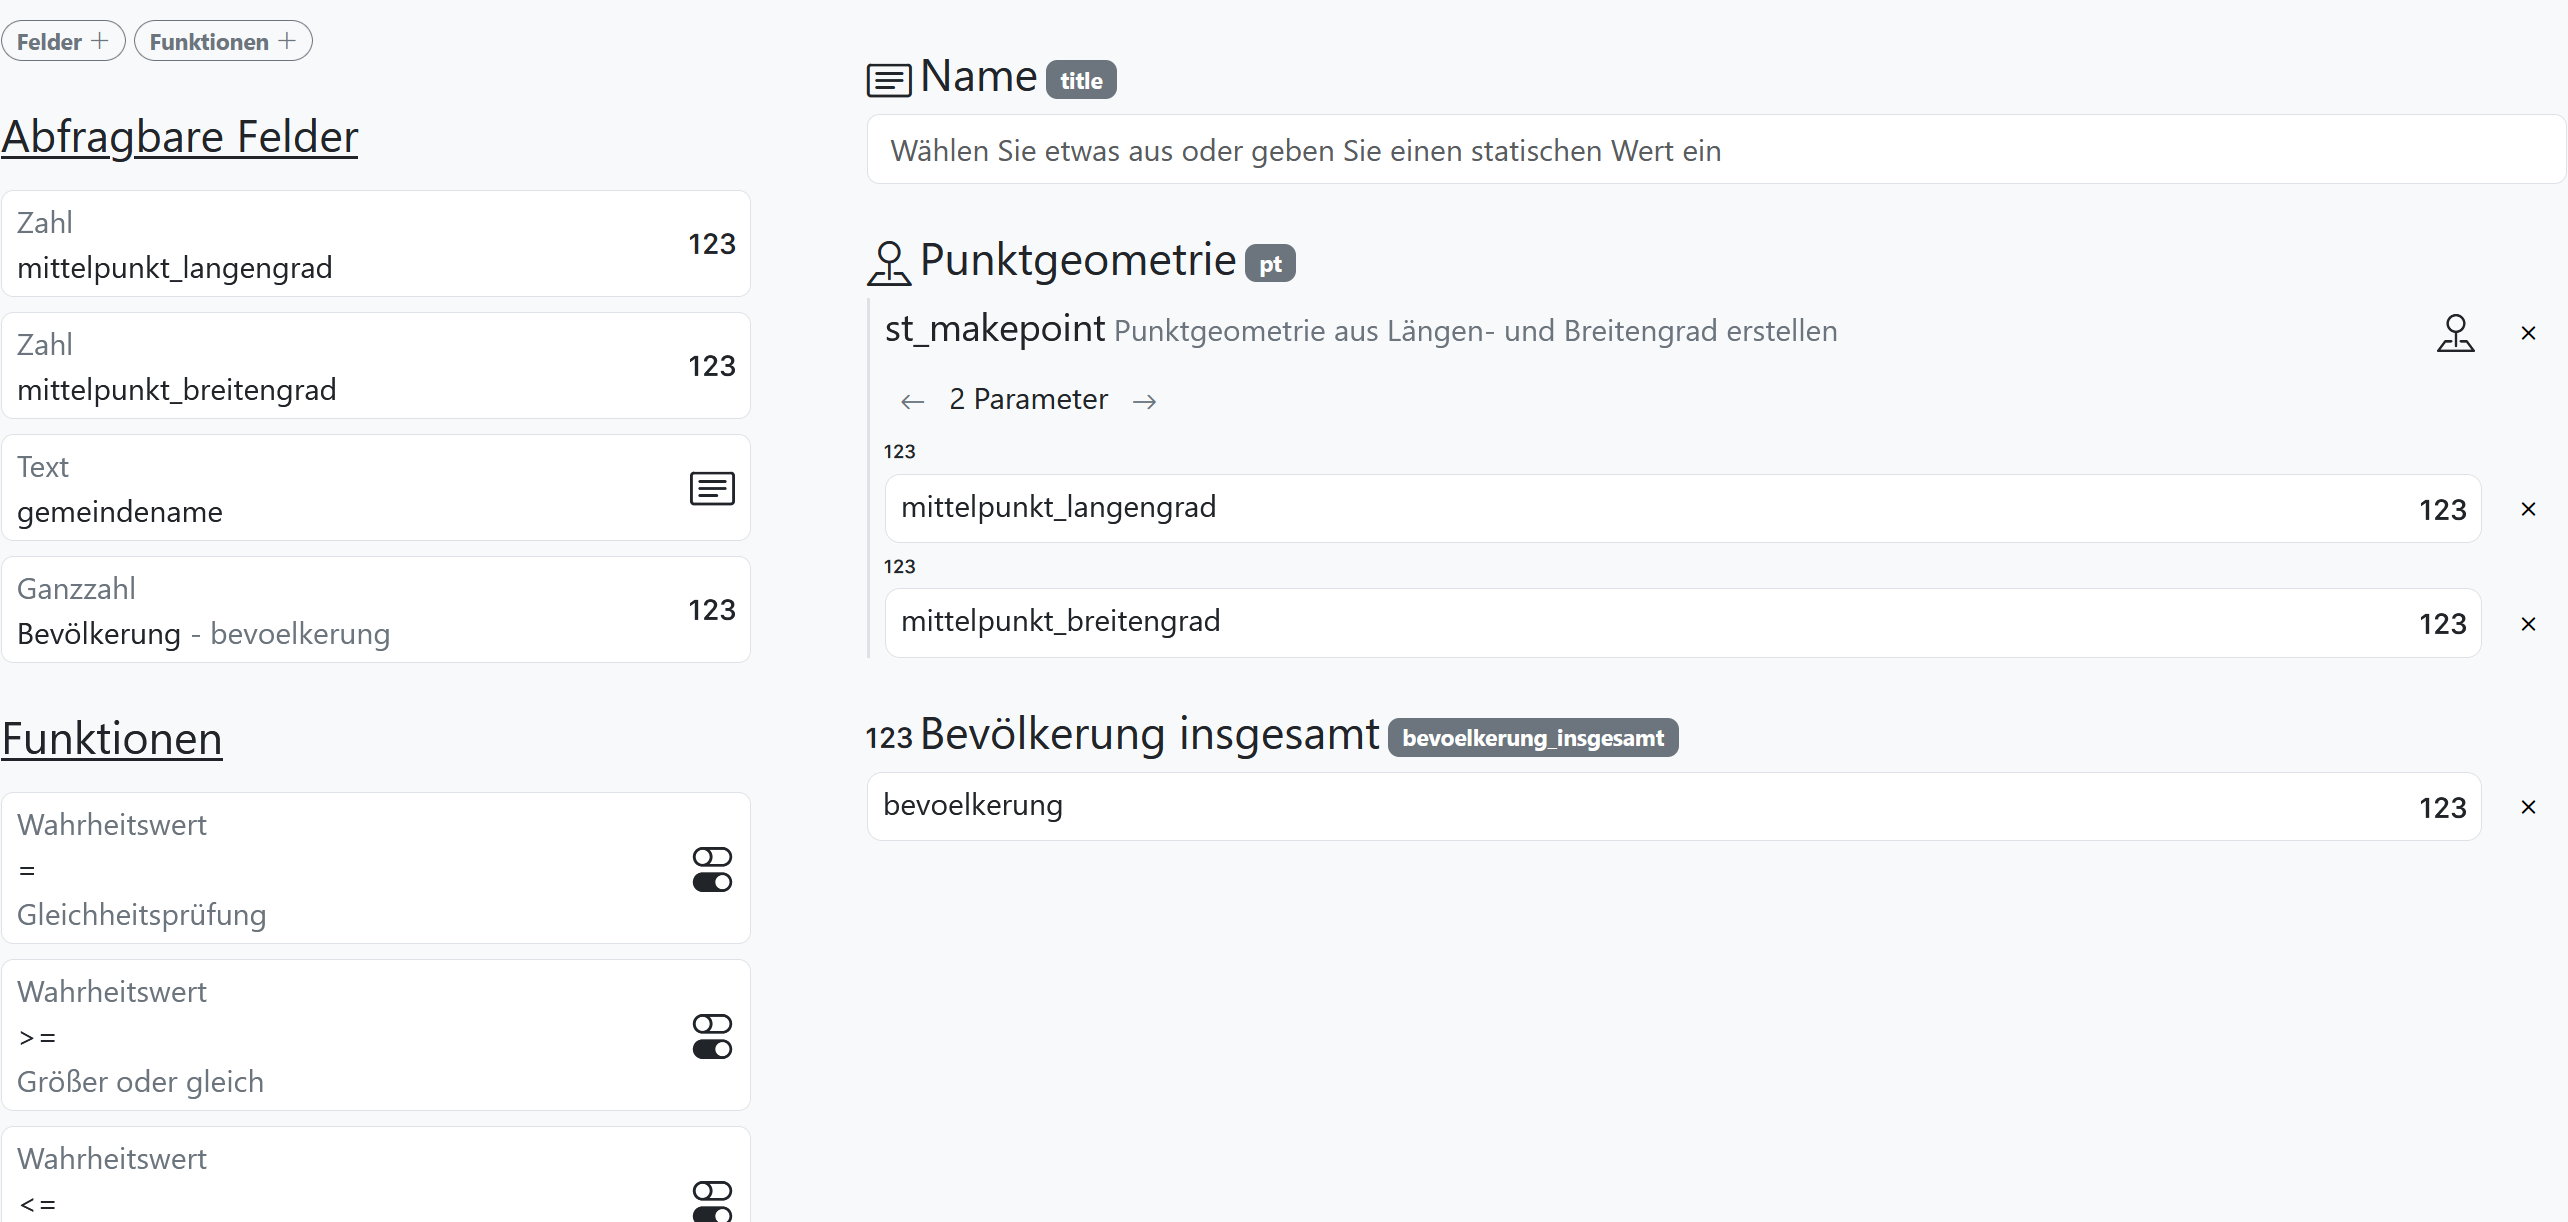
\includegraphics[width=0.95\textwidth]{assets/buffet-simple.png}
    \end{center}
    \caption{Bearbeitung einer Konvertierung im Block-Editor.}
  \end{figure}

\end{frame}

\begin{frame}
  % \frametitle{\currentsectionname{} (cont.)}

  \begin{figure}
    \centering
\begin{tikzpicture}
  \tikzset{icon/.style={outer xsep=4.5em, outer ysep=1em, minimum height=3em}}
  \tikzset{label/.style={font=\footnotesize}}
  \node [icon] (text)  at (0, 0)       {\includesvg[width=2em]{assets/bi-card-text.svg}};
  \node [icon] (int)   at (text.east)  {\includesvg[width=2em]{assets/bi-123.svg}};
  \node [icon] (float) at (int.east)   {\includesvg[width=2em]{assets/bi-123.svg}};
  \node [icon] (bool)  at (float.east) {\includesvg[width=2em]{assets/bi-toggles.svg}};
  \node [icon] (dt)    at (bool.east)  {\includesvg[width=2em]{assets/bi-calendar-week.svg}};
  \node [icon] (geom)  at (dt.east)    {\includesvg[width=2em]{assets/bi-pin-map.svg}};
  \node [label] at (text.south)  {Text};
  \node [label] at (int.south)   {Ganzzahl};
  \node [label] at (float.south) {Gleitkommazahl};
  \node [label] at (bool.south)  {Boolean};
  \node [label] at (dt.south)    {Datum/Zeit};
  \node [label] at (geom.south)  {Geometrie};
\end{tikzpicture}

    \caption{Die im Block-Editor verwendeten Symbole für Datentypen.}
  \end{figure}

  \begin{itemize}
    \item Verwechslung von Ganzzahl und Gleitkommazahl
    \item Symbol für Boolean wurde als Schaltflächen identifiziert
  \end{itemize}

  \Note{
    \item Verwechslung auch von Menschen mit Programmierkenntnissen
    \item Boolean-Problem Oft schon beim ersten Eindruck genannt
  }

\end{frame}

% \begin{frame}
%   % \frametitle{\currentsectionname{} (cont.)}
%
%   \begin{itemize}
%     \item Der Datentyp von Szenario-Feldern muss im Vorhinein bekannt sein und ausgewählt werden.
%     \item Das Dropdown-Menü wurde nicht immer sofort gefunden.
%   \end{itemize}
%
%   \begin{figure}
%     \begin{center}
%       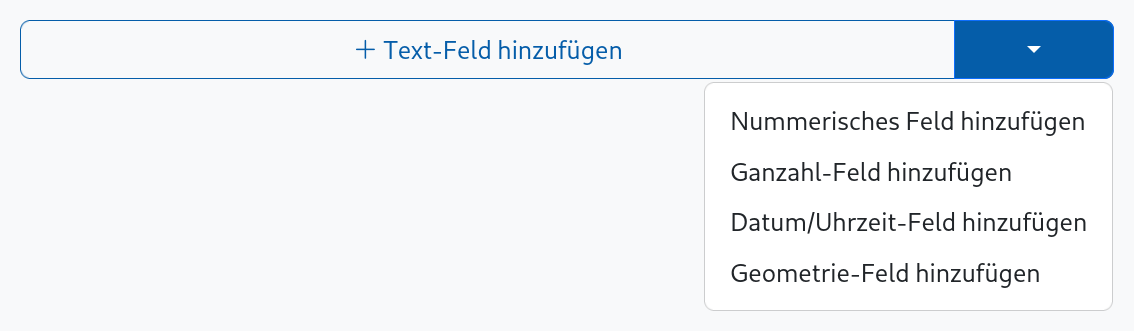
\includegraphics[width=0.95\textwidth]{assets/datatype-dropdown.png}
%     \end{center}
%     \caption{Dropdown-Menü zum Auswählen des Datentyps von Feldern.}
%   \end{figure}
%
% \end{frame}

\begin{frame}
  \frametitle{weitere aufgetretene Probleme}


  \begin{itemize}
    \item Interaktion
          \begin{itemize}
            \item Ersetzen von Einträgen
            \item Drag\&Drop
            \item Überladungen
          \end{itemize}
    \item Darstellung
          \begin{itemize}
            \item Konsistente Darstellung von Attributen
            \item Benennung von Speichern-Button und Auswahlmenü
          \end{itemize}
    \item Inhalt
          \begin{itemize}
            \item Details zu Parametern und Funktionen
            \item Zugriff auf Quelldaten
          \end{itemize}
  \end{itemize}

  \Note{
    \item Details: Längen und Breitengrad
  }

\end{frame}

\section{Diskussion}
\begin{frame}
  \frametitle{\currentsectionname}
  \note{
    \begin{itemize}
    \end{itemize}
  }
\end{frame}

\section*{\ShortTitle}
\subsection*{Literatur}
\begin{frame}
  \frametitle{\currentsectionname}
  \printbibliography{}
\end{frame}

\end{document}
